%%%%%%%%%%%%%%%%%%%%%%%%%%%%%%%%%%%%%%%%%
% Programming/Coding Assignment
% LaTeX Template
%
% This template has been downloaded from:
% http://www.latextemplates.com
%
% Original author:
% Ted Pavlic (http://www.tedpavlic.com)
%
% Note:
% The \lipsum[#] commands throughout this template generate dummy text
% to fill the template out. These commands should all be removed when 
% writing assignment content.
%
% This template uses a Perl script as an example snippet of code, most other
% languages are also usable. Configure them in the "CODE INCLUSION 
% CONFIGURATION" section.
%
%%%%%%%%%%%%%%%%%%%%%%%%%%%%%%%%%%%%%%%%%

%----------------------------------------------------------------------------------------
%	PACKAGES AND OTHER DOCUMENT CONFIGURATIONS
%----------------------------------------------------------------------------------------

\documentclass{article}
\usepackage[hangul]{kotex}
\usepackage{fancyhdr} % Required for custom headers
\usepackage{lastpage} % Required to determine the last page for the footer
\usepackage{extramarks} % Required for headers and footers
\usepackage[usenames,dvipsnames]{color} % Required for custom colors
\usepackage{graphicx} % Required to insert images
\usepackage{listings} % Required for insertion of code
\usepackage{courier} % Required for the courier font
\usepackage{lipsum} % Used for inserting dummy 'Lorem ipsum' text into the template
\usepackage{amsthm,amsmath}
\usepackage{algorithm, algpseudocode}
\usepackage{verbatim} % for commment, verbatim environment
\usepackage{spverbatim} % automatic linebreak verbatim environment
\usepackage{listings}
\DeclareGraphicsExtensions{.pdf,.png,.jpg}

% Margins
\topmargin=-0.45in
\evensidemargin=0in
\oddsidemargin=0in
\textwidth=6.5in
\textheight=9.0in
\headsep=0.25in

\linespread{1.1} % Line spacing

% Set up the header and footer
\pagestyle{fancy}
\lhead{}
\chead{나는코더다 2016 송년대회} % Top center head
\rhead{2016년 12월 12일 월요일} % Top right header
\lfoot{\lastxmark} % Bottom left footer
\cfoot{} % Bottom center footer
\renewcommand\headrulewidth{0.4pt} % Size of the header rule
\renewcommand\footrulewidth{0.4pt} % Size of the footer rule

\setlength\parindent{0pt} % Removes all indentation from paragraphs

%----------------------------------------------------------------------------------------
%	CODE INCLUSION CONFIGURATION
%----------------------------------------------------------------------------------------


\setcounter{secnumdepth}{0} % Removes default section numbers
\newcounter{homeworkProblemCounter} % Creates a counter to keep track of the number of problems



%----------------------------------------------------------------------------------------
%	TITLE PAGE
%----------------------------------------------------------------------------------------

%----------------------------------------------------------------------------------------

\begin{document}
\begin{titlepage}
	\centering
	{2016년 12월 12일 월요일\par}
	{경기과학고등학교 32기 구재현\par}
	\vspace{2cm}
	{\huge 나는코더다 2016 송년 대회 \par}
	\vspace{4cm}
	{\Large 문제 배열은 난이도 순이 아닙니다. 모든 문제를 읽는 것을 권장합니다.\par}
	\vspace{4cm}
	\label{my-label}
	\begin{tabular}{|l|l|l|l|}
		\hline
		& 문제 이름                  & 시간 제한 & 메모리 제한 \\ \hline
		A & 버스 여행               & 1초    & 128MB  \\ \hline
		B & 큐브러버                   & 1초    & 128MB  \\ \hline
		C & 크리스 마틴                 & 1초    & 128MB  \\ \hline
		D & 내일 할거야                 & 2초    & 128MB  \\ \hline
		E & 풍선 놀이                  & 1초    & 128MB  \\ \hline
		F & 장비를 정지합니다               & 1초    & 256MB  \\ \hline
		G & 순열 그래프의 연결성 판별         & 2초    & 256MB  \\ \hline
		H & 두더지 잡기                & 1초    & 256MB  \\ \hline
		I & 수열                     & 1초    & 256MB  \\ \hline
		J & 비무장 지대 & 3초    & 256MB  \\ \hline
		K & 그래프와 쿼리                  & 2초    & 256MB  \\ \hline
	\end{tabular}

\end{titlepage}

%----------------------------------------------------------------------------------------
%	PROBLEM 1
%----------------------------------------------------------------------------------------

% To have just one problem per page, simply put a \clearpage after each problem


\section{문제 A. 버스 여행}
20xx년, 경기과학고등학교는 국내 최대의 프로그래밍 대회인 ACM-ICPC Suwon Regional을 주최하게 되었다! 이번 수원 리저널에서는, 단순한 대회 주최 뿐만 아니라, 참가자들을 위한 수원시 버스 여행까지 계획되어 있고, 재현이는 이 버스 여행의 자세한 경로를 계획할 예정이다. \newline

비록 2016년의 수원시는 정돈된 시가지하고는 거리가 멀지만, 20xx년의 수원시는 동-서 거리와 남-북 거리로 잘 정돈된 그리드 형태의 시가지를 가지고 있다. 서로 인접한 평행한 거리들은 100m 간격으로 떨어져 있다. 관광 명소는 항상 이러한 거리들의 교차로에 있는데, 재현이는 여행사를 통해서 각각의 관광 명소의 건설 시기 $a_{i, j}$와 매력도 $c_{i, j}$를 알고 있다. \newline

재현이는 버스 여행을 통해 순서대로 여러 관광 명소를 방문할 계획이며, 이 때의 매력도의 합을 최대화하려고 한다. 한편, 이번 버스 여행의 테마는 수원시의 역사이기 때문에, 건설 시기가  증가하는 (같아서는 안된다!) 순으로 관광 명소를 방문하려고 한다. 또한, 수원시의 경치는 너무나도 아름다워서, 사람들은 버스 안에서 수원시의 경치를 감상하는 것을 즐긴다. 때문에, 두 관광 명소 사이를 이동하는 와중에도 매력도가 100m마다 1씩 증가한다. \newline

재현이는 아무 관광 명소에서 시작해서, 중간에 여러 관광 명소를 들린 후, 아무 관광 명소에서 도착하는 여행 계획을 만들려고 한다. 가능한 여행 계획 중, 매력도의 합의 최댓값은 얼마인가? 버스는 두 관광 명소 사이를 최단 거리로 움직이며, 버스가 움직이는 동안 지나쳤던 관광지는 방문했다고 치지 않는다. 


\subsection{입력}
첫번째 줄에는 동-서 거리와 남-북 거리의 개수인 $n$, $m$ 이 주어진다. ($2 \leq n, m \leq 1000$) \newline

이후 $n$ 개의 줄에 각각의 관광 명소의 건설 시기가 주어진다. 이 중 $i$번째 줄에는 $m$개의 정수 $a_{i, j}$ ($0 \leq a_{i, j} \leq 10^6$)가 주어지며, $i$번 동-서 거리와 $j$번 남-북 거리의 교차로를 의미한다. $a_{i, j} = 0$ 일 경우, \textbf{해당 거리의 교차로에는 관광 명소가 없다.} 관광 명소는 하나 이상 존재한다.\newline

이후 $n$ 개의 줄에 각각의 관광 명소의 매력도가 주어진다. 이 중 $i$번째 줄에는 $m$개의 정수 $c_{i, j}$ ($0 \leq c_{i, j} \leq 10^9$) 가 주어지며, $i$번 동-서 거리와 $j$번 남-북 거리의 교차로에 있는 관광 명소의 매력도를 뜻한다. 만약에 해당 교차로에 관광 명소가 없다면, $c_{i, j} = 0$ 임이 보장된다. 

\subsection{출력}
가능한 여행 계획 중, 매력도의 합의 최댓값을 출력하라.

\subsection{예제}
입력
\bgroup\obeylines
\texttt{4 5
1 2 6 0 2
1 3 4 0 4
0 0 4 0 3
2 2 0 0 4
1 3 5 0 2
2 8 1 0 2
0 0 3 0 4
0 5 0 0 3 \newline \newline}
\egroup

출력
\bgroup\obeylines
\texttt{39 \newline}
\egroup

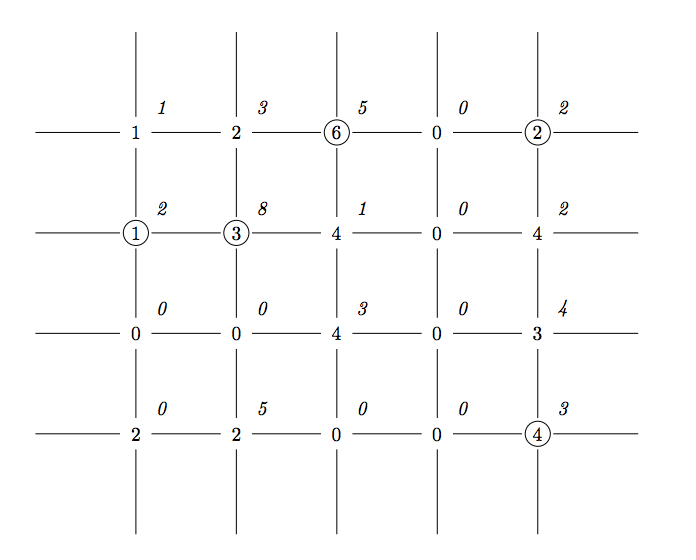
\includegraphics{fig1.png}\newline
\textbf{예제 설명:} 재현이는 $(2, 1) \rightarrow (1, 5) \rightarrow (2, 2) \rightarrow (4, 5) \rightarrow (1, 3)$ 순으로 관광 명소를 방문한다. 관광 명소의 매력도의 합은 $2 + 2 + 8 + 3 + 5 = 20$ 이고, 이동 중에 쌓은 매력도의 합은 $5 + 4 + 5 + 5 = 19$ 이다. 고로 총 매력도의 합은 39이다. 


\newpage
%----------------------------------------------------------------------------------------
%	PROBLEM 2
%----------------------------------------------------------------------------------------


\section{문제 B. 큐브러버}
지학이는 3차 다항식(cubic polynomial)을 좋아하는 잘 알려진 \textbf{cubelover} 이다. \newline

어느 화창한 봄날, 지학이는 아파트 놀이터에서 승현이가 길이 $n$의 정수 수열 $x_1, x_2, ..., x_n$ 을 가지고 노는 것을 보았다. 지학이는 그 아파트의 짱이었고, 승현이보다 45일이나 먼저 태어난 형이었다. 지학이는 승현이를 보자마자  갖고 놀던 수열을 빼앗아 갔다. \newline

승현이는 그 자리에서 엉엉 울기 시작했고, 마음이 약해진 지학이는 승현이가 $1 \leq i \leq n$인 모든 정수 $i$에 대해 $x_i = ai^3 + bi^2 + ci + d$를 만족하는 실수 $a$, $b$, $c$, $d$ 를 찾으면 수열을 돌려주겠다고 약속했다. (사실 3차 다항식이라 $a \neq 0$이어야 하긴 하는데, 지학이는 그 정도로 엄밀하게 굴고 싶진 않은 모양이다.) \newline

간만에 학교를 나와 외출을 즐기고 있는 당신은, 울고 있는 승현이와 눈을 마주쳤다. 승현이는 여러분에게 곧장 달려와서, 빨리 그러한 실수 $a$, $b$, $c$, $d$ 를 찾아달라고 졸랐다. 당신은 과연 승현이의 눈물을 닦아 줄 수 있는가?

\subsection{입력}
이 문제는 한 입력에 여러 개의 테스트 케이스가 주어진다. 첫번째 줄에 그러한 테스트 케이스의 개수 $T$ ($1 \leq T \leq 1000$) 가 주어진다. \newline

이후 $T$개의 줄이 주어진다. 첫번째로 수열의 길이인 정수 $n$ ($1 \leq n \leq 500$) 이 주어진다. 이후 $n$ 개의 정수가 주어진다. 이 중 $i$번째 정수는 $x_i$ ($0 \leq x_i \leq 50,000,000$) 를 뜻한다.


\subsection{출력}
$T$개의 줄에 걸쳐, 만약에 승현이가 원하는 실수 $a$, $b$, $c$, $d$가 존재한다면 YES, 존재하지 않는다면 NO를 출력한다.

\subsection{예제}
입력
\bgroup\obeylines
\texttt{3
	1 3
	5 0 1 2 3 4
	5 0 1 2 4 5	\newline}
\egroup

출력
\bgroup\obeylines
\texttt{YES
	YES
	NO \newline}
\egroup

\textbf{예제 설명:} 첫번째 테스트 케이스에서, 가능한 답 중 하나는 $a = 0$, $b = 0$, $c = 0$, $d = 3$ 이다.



\newpage

%----------------------------------------------------------------------------------------
%	PROBLEM 3
%----------------------------------------------------------------------------------------


\section{문제 C. 크리스 마틴}
미친 과학자 창호는 어젯 밤 구재현을 납치해서, 구재현의 DNA를 추출했다. 인간의 DNA의 길이는 $n$이며, $A$, $C$, $G$, $T$ 4개의 염색체로 구성되어 있다. \newline

창호는 매일 자신을 놀리던 구재현을 좋아하지 않고, 대신 잘 생긴 콜드플레이의 크리스 마틴을 더 좋아한다. 이러한 경험을 토대로 창호는 이론을 하나 만들었다. 창호의 이론에 따르면, 구재현의 DNA와의 유사도가 최소인 DNA가 크리스 마틴의 DNA이다. \newline

두 DNA의 유사도는, 두 DNA 간의 최장 공통 부분 수열(LCS)의 길이를 뜻한다. 어떠한 DNA의 부분 수열은, 그 DNA에서 0개 이상의 원소를 제거해서 만들 수 있는 또 다른 DNA 수열을 뜻한다. 두 DNA $A$, $B$의 최장 공통 부분 수열은, $A$와 $B$의 부분 수열이면서, 길이가 최대인 수열들을 뜻한다. \newline

사실 잘 몰랐겠지만, 여러분도 지금 창호에게 납치되어 있다. 크리스 마틴의 DNA를 구하지 못하면 여러분에게 무슨 일이 일어날 지 모른다. 빨리 크리스 마틴의 DNA를 구하자. 가능한 답이 여러 가지일 경우, 아무거나 출력하면 된다.

\subsection{입력}
첫번째 줄에 인간 DNA의 길이 $n$이 주어진다. ($1 \leq n \leq 10,000$) 이 주어진다. \newline

이후 길이 $n$의 DNA 문자열이 주어진다. 문자열의 모든 문자는 $A$, $C$, $G$, $T$ 넷 중 하나다.

\subsection{출력}
첫번째 줄에 최소 유사도 $c$ 를 출력한다. \newline

두번째 줄에 이를 만족하는 길이 $n$의 문자열을 출력한다. 가능한 답이 여러개 일 경우, 아무거나 출력하면 된다.

\subsection{예제}
입력
\bgroup\obeylines
\texttt{4
	GACT	\newline}
\egroup

출력
\bgroup\obeylines
\texttt{1
	TCAG\newline}
\egroup

\newpage

%----------------------------------------------------------------------------------------
%	PROBLEM 4
%----------------------------------------------------------------------------------------


\section{문제 D. 내일 할거야}
아 과제 하기 싫다. 아무 것도 안 하고 싶다. 더 적극적이고 격렬하게 아무 것도 안 하고 싶다. \newline

있잖아. 내가 아까 책상에다가 $n$개의 과제 목록을 적어놨어. 각각의 과제 $i$는 $d_i$ 일이 걸리고, 오늘로부터 $t_i$ 일 안에 끝내야 해. 그러니까 오늘이 0일이면, $t_i$일이 끝나기 전에 제출이야. 과제는 한번 시작하면 쉬지 않고 계속 해야 해. 안 그러면 머리 아파 지거든. \newline

근데 있잖아. 내가 지금 너무, 너무 아무 것도 안 하고 싶어. 그래서 오늘은 아무 것도 안 할 거야. 더 중요한 게 뭔지 알아? 사실 나 내일도, 모레도, 아무 것도 안 하고 싶어. 한 며칠 동안은 계속 아무 것도 안하려고. 아. 과제가 있을 때 내가 내일부터 연속으로 최대 며칠동안 놀 수 있는지 궁금하다. 궁금하긴 한데, 난 아무 것도 안 하고 싶어. \newline

좋은 생각이 났다. 너희가 이걸 대신 구해주면, 내가 너희의 맞은 문제 수를 하나 올려줄게.

\subsection{입력}
첫째 줄에는 과제의 개수인 정수 $n$ ($1 \leq n \leq 10^6$)이 주어진다. \newline

이후 $n$개의 줄에 각각의 과제를 나타내는 두 정수 $d_i$, $t_i$ ($1 \leq d_i, t_i \leq 10^9$)가 순서대로 주어진다. 오늘은 0일이다. \newline

모든 입력에 대해, 오늘 아무 것도 안 해도 과제를 마무리 할 수 있는 방법이 존재함이 보장된다.

\subsection{출력}
내일(1일)부터 연속으로 최대 며칠 동안 놀 수 있는지를 출력한다. 가령, 답이 0이면, 내일 과제를 해야 하며, 1이면, 모레에 과제를 해야 한다.

\subsection{예제}
입력
\bgroup\obeylines
\texttt{3
	2 8
	1 13
	3 10 \newline}
\egroup

출력
\bgroup\obeylines
\texttt{5\newline}
\egroup

\textbf{예제 설명:} 1--5일에는 놀고, 6--7일에는 1번째 과제를, 8--10일에는 3번째 과제를 한다. 11--12일에는 놀고, 13--13일에 2번째 과제를 한다.

\newpage


%----------------------------------------------------------------------------------------
%	PROBLEM 5
%----------------------------------------------------------------------------------------


\section{문제 E.  풍선 놀이}
매년 가을 대전에서 열리는 대학생 프로그래밍 대회의 묘미 중 하나는 풍선 놀이이다. 시상식에서 스코어보드 공개를 기다리다가 심심해지면, 주위에 있는 풍선을 엮어서, 대회장을 가로지르는 긴 풍선 줄을 만드는 것이다! 이 풍선을 아치형으로 단상 위에 올리면, 본인의 잉여로움을 참가자들에게 뽐낼 수 있는 기회가 생긴다. \newline

심심해진 재현이와 한필이는 풍선 놀이를 위해서 기다란 풍선 줄을 가져왔다. 풍선 줄에는 풍선을 매달 수 있는 $N$개의 슬롯이 있으며, 각 슬롯은 1번부터 $N$번까지 번호가 붙어있다. 풍선 줄에, 한필이는 $Q$번에 걸쳐서 규칙적으로 풍선을 꽂았다. 예를 들면, '1번 슬롯부터 3개씩 띄어서 풍선을 놓자' 라고 한필이가 생각했다면, 1, 4, 7, 10, ... 번째 슬롯에 풍선을 놓으며, 슬롯의 번호가 $N$을 초과하면 풍선을 놓는 것을 그만 둔다. 이미 풍선이 놓여진 슬롯은 건너 뛴다. \newline

$Q$번에 걸친 풍선 설치가 끝난 후, 한필이는 어떤 슬롯들이 비어 있는 것을 확인했다. 이 슬롯을 메꾸는 풍선을 가져오기 위해서, 총 몇개의 슬롯이 비었는지를 계산해주자. 

\subsection{입력}
첫번째 줄에 슬롯 수 $N$과 풍선들을 꽂는 횟수 $Q$가 주어진다. ($1 \leq N \leq 10,000$, $1 \leq Q \leq 100$) \newline

이후 $Q$개의 줄에 풍선을 꽂는 방법이 주어진다. 방법은 두 정수 $L$과 $I$로 주어지며, "$L$번 슬롯부터 $I$개씩 띄어서 풍선을 놓자" 라는 뜻이다. ($1 \leq L, I \leq N$)

\subsection{출력}
비어있는 슬롯의 개수를 출력하라.

\subsection{예제}
입력
\bgroup\obeylines
\texttt{30 3
	1 3
	3 7
	1 4		\newline}
\egroup

출력
\bgroup\obeylines
\texttt{13	\newline}
\egroup

\textbf{예제 설명 : } 초기 빈 풍선 줄은 다음과 같다. 

\texttt{
	. . . . . . . . . . . . . . . . . . . . . . . . . . . . . . \newline
}

한필이가 1번 슬롯부터 3개씩 띄어서 R 풍선을 설치했다.

\texttt{
	R . . R . . R . . R . . R . . R . . R . . R . . R . . R . . \newline
}

3번 슬롯부터 7개씩 띄어서 B 풍선을 설치했다.

\texttt{
	R . B R . . R . . R . . R . . R B . R . . R . B R . . R . . \newline
}

1번 슬롯부터 4개씩 띄어서 D 풍선을 설치했다. 

\texttt{
	R . B R D . R . D R . . R . . R B . R . D R . B R . . R D . \newline
}

최종적으로 13개의 슬롯이 빈다.
\newpage


%----------------------------------------------------------------------------------------
%	PROBLEM 6
%----------------------------------------------------------------------------------------


\section{문제 F.  장비를 정지합니다}
졸업논문을 완성하지 못한 형서는 학교에 대한 테러 계획을 세웠다. 고급정보과학 시간에 몰래 형서가 제작한 기계는, 전원을 켠 순간부터 폭주하기 시작해서 온 학교를 쑥대밭으로 만들고 있다. 으악! \newline

학교를 살려내기 위해서, 박종화 선생님은 형서의 설계도를 입수했다. 설계도에 의하면, 폭주 기계에는 $n$개의 장비가 존재하며, 현재 1번 장비만이 폭주하고 있다. 장비를 정지시키기 위해서는, 박종화 선생님이 각각의 장비에 전기 충격을 가해야 한다. \newline

설계도에 의하면, 전기 충격에는 \textbf{약한 충격}과 \textbf{강한 충격}이 있다. $i$번 장비에 약한 충격을 가하는 데는 $u_i$ 와트의 전력이 필요하며, 강한 충격을 가하는 데는 $z_i$ 와트의 전력이 필요하다. ($u_i < z_i$) 약한 충격과 강한 충격 모두 $i$번 장비를 정지시키지만, 약한 충격을 받았을 때는, $r_i$ 개의 특정한 장비들이 다시 작동을 시작하게 된다! 각각의 장비에 대해서, 이러한 특정한 장비들은 $g_{i, 1}, ..., g_{i, r_i}$ 와 같은 리스트로 표현 가능하며, 이 리스트 역시 설계도에 적혀 있다. \newline

박종화 선생님은 모든 장비를 정지하려고 한다. 하지만, 학교는 난장판이 되었고, 공급받을 수 있는 전력량에는 한계가 있다. 박종화 선생님은 전기 충격에 사용한 전력의 합의 최솟값을 구하려고 한다. 힘을 합쳐서 박종화 선생님을 도와드리자. 

\subsection{입력}
첫번째 줄에는 장비의 개수를 뜻하는 정수 $n$이 주어진다. ($1 \leq n \leq 200,000$). \newline

이후 $n$개의 줄에 장비의 정보가 순서대로 주어진다. 이 중 $i$번째 줄은 장비 $i$의 정보를 나타낸다. 각각의 줄에는 먼저 세 정수 $u_i$, $z_i$, $r_i$ 가 주어지며 ($1 \leq u_i < z_i \leq 10^9$, $1 \leq r_i < n$), 이후 $r_i$개의 정수 $g_{i, 1}, ..., g_{i, r_i}$ ($1 \leq g_{i, j} \leq n$)가 주어진다. 모든 $i$에 대해 $r_i$의 합은 $10^6$을 넘지 않는다. \textbf{다시 작동을 시작하는 장비의 리스트에, 같은 원소가 여러 번 등장할 수 있으며, 이 때는 해당 장비를 등장 횟수만큼 종료해야 한다.}

\subsection{출력}
모든 장비를 정지하기 위해 필요한 전력량의 최솟값을 출력하라.

\subsection{예제}
입력
\bgroup\obeylines
\texttt{4
	4 27 3 2 3 2
	3 5 1 2
	1 13 2 4 2
	5 6 1 2\newline}
\egroup

출력
\bgroup\obeylines
\texttt{26	\newline}
\egroup

\newpage

%----------------------------------------------------------------------------------------


%----------------------------------------------------------------------------------------
%	PROBLEM 7
%----------------------------------------------------------------------------------------

\section{문제 G.  순열 그래프의 연결성 판별}
크기 $n$의 순열은, $1$부터 $n$까지의 정수가 정확히 한 번 등장하는 길이 $n$의 수열을 뜻한다. 이 순열을 $a_1, a_2, ..., a_n$으로 표기하자. 순열 $a$를 통해서 \textbf{순열 그래프}를 만들 수 있다. 순열 그래프는 $1, 2, ..., n$의 번호를 가진 $n$개의 정점으로 이루어진 무방향 그래프이다. 순열 그래프의 두 정점 쌍 $i, j$ ($1 \leq i < j \leq n$) 는 $a_i > a_j$ 일때 간선으로 연결되어 있다.  \newline

순열 그래프의 연결성을 판별하기 위해서, 당신은 순열 그래프를 다음과 같은 알고리즘으로 탐색해야 한다. 
\begin{enumerate}  
	\item 1번 정점부터 순서대로 $n$번 정점까지 순회한다. 현재 처리 중인 정점을 $i$ 번 정점이라고 하자.
	\item $i$번 정점이 이전에 탐색되었다면, 넘어간다. 그렇지 않다면, $i$번 정점과 연결된 모든 정점을 탐색한 후, 탐색한 정점을 모아 집합을 하나 만든다.
	\item 최종적으로, 구한 집합의 총 개수와, 각 집합의 정보를 출력한다.  
\end{enumerate}

알고리즘을 읽은 동욱이는, 이 문제가 그래프의 연결 컴포넌트를 구하는 쉬운 문제임을 알게 되었다. 동욱이는 재현이에게 "이거 깊이 우선 탐색으로 풀면 돼?" 라고 물었다. 재현이는 아무 대답도 하지 않았다. 당신은 어떻게 생각하는가?

\subsection{입력}
첫번째 줄에 순열의 길이 $n$ ($1 \leq n \leq 1,000,000$)이 주어진다. \newline

두번째 줄에 $n$개의 공백으로 구분된 정수가 주어진다. 순열의 원소 $a_1, a_2, ..., a_n$ 을 뜻한다.

\subsection{출력}
첫번째 줄에 구한 집합의 개수 $m$을 출력한다. \newline

이후 $m$개의 줄에 걸쳐 각각의 집합을 출력한다. 첫번째로 집합의 크기 $s_i$를 출력하고, 이후 그 집합에 속한 $s_i$개의 정점의 번호를 공백으로 구분하여 출력한다. 정점의 번호는 오름차순으로 출력한다. \newline

여러 개의 집합을 출력할 때, 집합에 속한 가장 작은 번호의 정점을 기준으로 오름차순으로 출력하라.

\subsection{예제}
입력
\bgroup\obeylines
\texttt{4
	2 3 1 4	\newline}
\egroup

출력
\bgroup\obeylines
\texttt{2
	3 1 2 3
	1 4	\newline}
\egroup

\textbf{예제 설명:} 예제의 순열 그래프를 그리면 다음과 같다.

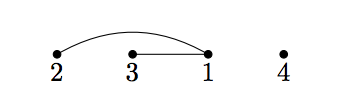
\includegraphics[scale=0.75]{fig2.png}

\newpage

%----------------------------------------------------------------------------------------
%	PROBLEM 8
%----------------------------------------------------------------------------------------

\section{문제 H.  두더지 잡기}
요즘 이상한 뉴스가 너무 많아서 그런지, 재현이의 성격은 점점 반사회적이고 폭력적으로 변했다. 얼마 전, 재현이는 결국 학교의 3D 프린터를 사용해서 모형 권총을 프린트하고, 혼자 이상한 게임을 하기 시작했다. \newline

재현이는 많은 두더지굴이 있는 잔디밭에서 게임을 시작했다. 잔디밭에는 $n$개의 두더지굴이 있으며, 두더지굴은 1번부터 $n$번까지 순서대로 번호가 부여되어 있다. 원형으로 늘어져 있으니, 1번 굴과 2번 굴, 2번 굴과 3번 굴, ..., $n$번 굴과 1번 굴은 인접해 있다. \newline

현재 각각의 굴에는 $a_i$ 마리의 두더지가 있고, 재현이는 모형 권총으로 이들을 쫓아낼 계획이다. 재현이가 모형 권총을 쏴서 $i$번 굴에 있는 두더지에게 겁을 주면, 그 굴에 있는 두더지들이 겁을 먹고 도망가게 된다. (모형이라 죽지는 않는다.) 뿐만 아니라, 그 굴과 인접한 양 옆 두개의 굴에 있는 두더지들도 겁을 먹어서, 인접한 굴로 이동하게 된다. 당연히, 인접한 굴이라 하면 $i$번 굴은 아니다. \newline

예를 들어, 10번 굴에 겁을 줬다면, 10번 굴에 있는 두더지는 모두 굴을 탈출하고, 9번 굴에 있는 두더지는 8번 굴로 도망가고, 11번 굴에 있는 두더지는 12번 굴로 도망간다. \newline

재현이는 3D 프린터로 $k$개의 총알을 만들었고, 최대한 많은 두더지를 쫓아내고 싶다. 총을 $k$번 이하로 사용했을 때, 최대 몇 마리의 두더지가 굴을 탈출하는가?

\subsection{입력}
첫번째 줄에 두더지굴의 수 $n$, 총의 최대 사용 가능 수 $k$가 주어진다. ($5 \leq n \leq 2000$, $1 \leq k \leq n$) \newline

이후 $n$개의 정수 $a_1, a_2, ..., a_n$가 주어진다. ($0 \leq a_i \leq 10^6$) $i$번째 굴에 $a_i$마리의 두더지가 산다는 것을 의미한다.


\subsection{출력}
총을 $k$번 이하로 사용했을 때, 탈출시킬 수 있는 두더지 수의 최댓값을 출력한다.

\subsection{예제}
입력
\bgroup\obeylines
\texttt{5 2
	6 1 5 3 4	\newline}
\egroup

출력
\bgroup\obeylines
\texttt{13	\newline}
\egroup

\textbf{예제 설명:} 초기 두더지 굴의 상태는 $[6, 1, 5, 3, 4]$ 이다. \newline

첫번째로, 재현이는 1번째 굴에 총을 쏴서, 6마리의 두더지를 탈출시킨다. 두더지 굴의 상태는 $[0, 0, 6, 7, 0]$이 된다. \newline

이제, 재현이는 4번째 굴에 총을 쏴서, 7마리의 두더지를 탈출시킨다. 총 13마리가 탈출한다.

\newpage

%----------------------------------------------------------------------------------------
%	PROBLEM 9
%----------------------------------------------------------------------------------------

\section{문제 I. 수열}
정수 수열 $a_1, a_2, ..., a_n$이 있을 때, $1 \leq i \leq n-k+1$ 인 모든 정수 $i$에 대해서, $a_{i} + a_{i+1} + ... + a_{i+k-1}$ 이 짝수라면, 이 수열을 $k$-짝합 수열이라고 정의한다. \newline

당신은 수열에 있는 몇 개의 원소를 원하는 정수로 바꿀 수 있다. 최소 몇 개의 원소를 바꿔야지 수열을 $k$-짝합 수열로 만들 수 있는가?

\subsection{입력}
첫번째 줄에는 정수 $n$, $k$가 주어진다. ($1 \leq k \leq n \leq 10^6$) \newline

두번째 줄에는 $n$개의 정수가 주어진다. 이 중 $i$ 번째 정수는 $a_i$($0 \leq a_i \leq 10^9$) 를 뜻한다.


\subsection{출력}
바꿔야 하는 원소의 최소 개수를 출력한다.

\subsection{예제}
입력1
\bgroup\obeylines
\texttt{8 3
	1 2 3 4 5 6 7 8	\newline}
\egroup

출력1
\bgroup\obeylines
\texttt{3\newline}
\egroup


입력2
\bgroup\obeylines
\texttt{8 3
	2 4 2 4 2 4 2 4\newline}
\egroup

출력2
\bgroup\obeylines
\texttt{0\newline}
\egroup

\newpage

%----------------------------------------------------------------------------------------
%	PROBLEM 10
%----------------------------------------------------------------------------------------

\section{문제 J. 비무장 지대}
서기 12117년, 남한과 북한은 한반도의 위대한 지성인 최석환 (gs12117) 선생을 기리기 위해서 통일을 선언했다.\newline

(1998년생 이원형과 아무 관계 없는) 대한민국의 이원형 장군은 조국의 사이버 국방을 책임지는 위대한 군인이다. 그는 지금 비무장 지대에 쌓여있는 지뢰를 어떻게 제거해야 하는지에 대해서 고민하고 있다. 비무장 지대는 0부터 $10^9$까지의 수직선으로 모델링할 수 있으며, 정확히 $N$($1 \leq N \leq 10^6$) 개의 지뢰가 묻혀 있으며, 이 중 $i$번째 지뢰는 $X_i$ ($0 \leq X_i \leq 10^9$)위치에 묻혀 있다. 지뢰가 묻혀있는 위치 $X_i$ 에서 이상이 감지된다면, 지뢰는 폭발한다. \newline

핵지뢰부터 갤럭시 노트 7까지, 다양한 형태의 폭탄이 비무장 지대에 묻혀 있기 때문에, 이들의 폭발 양상은 다른 형태를 띈다. $i$번째 지뢰는 왼쪽으로 $L_i$, 오른쪽으로 $R_i$ 만큼의 범위로 폭발하며, 이는 $[X_i - L_i, X_i + R_i]$ 폐구간이 지뢰의 폭발 범위라는 것이다. ($1 \leq L_i, R_i \leq 10^9$) 지뢰의 폭발은 연속적인 지뢰의 폭발을 낳는다. 아직 폭발되지 않은 다른 지뢰의 중심이 폭발 범위 안에 들어간다면, 이 지뢰 역시 폭발하게 된다. \newline

이원형 장군은 1개의 지뢰를 시범적으로 터트릴 예정이지만, 비무장 지대에는 다양한 문화 유산과 멸종위기 동물들이 살고 있다. 이원형 장군은 이를 최대한 보호하기 위해서, 사전 조사를 거치려고 한다. 이원형 장군은 $M$($1 \leq M \leq 300,000$) 개의 보호 구역 위치 $C_i$ ($0 \leq C_i \leq 10^9$)를 지정해 놓았으며, 각각의 보호 구역에 대해서, 해당 보호 구역을 파괴할 수 있는 지뢰의 개수를 구하고 싶어한다. 해당 보호 구역을 파괴할 수 있는 지뢰라는 것은, 해당 지뢰를 터트렸을 때, 연속적인 폭발 반응의 결과로 해당 보호 구역이 어떤 폭발한 지뢰의 폭발 범위 안에 들어갔음을 뜻한다. \newline

젊은 시절 유능한 코이충으로 각광받던 이원형 장군이었지만, 지금은 대국민 담화를 준비해야 해서 너무나도 바쁘다. 여러분들이 이원형 장군을 대신해서 문제를 풀어주자.

\subsection{입력}
첫번째 줄에 지뢰의 수 $N$, 보호구역의 수 $M$이 주어진다. ($1 \leq N \leq 10^6$, $1 \leq M \leq 300,000$) \newline

이후 $N$ 개의 줄이 주어진다. 이 중 $i$번째 줄에는, $i$번 지뢰의 위치, 폭발 범위를 나타내는 세 정수 $X_i, L_i, R_i$가 순서대로 주어진다. ($0 \leq X_i \leq 10^9$, $1 \leq L_i, R_i \leq 10^9$) \newline

이후 $M$ 개의 줄이 주어진다. 이 중 $i$번째 줄에는, 보호 구역의 위치인 정수 $C_i$ 가 주어진다. ($0 \leq C_i \leq 10^9$)

\subsection{출력}
$M$ 개의 줄에 걸쳐 각각의 보호 구역을 파괴할 수 있는 지뢰의 수를 하나의 정수로 출력한다. 

\subsection{예제}
입력
\bgroup\obeylines
\texttt{4 4
	10 5 12
	4 5 6
	15 1 1
	20 10 80
	101
	100
	0
	14\newline}
\egroup

출력
\bgroup\obeylines
\texttt{0
	3
	1
	4\newline}
\egroup


\textbf{예제 설명:} 101에 있는 보호 구역을 터트릴 수 있는 폭탄은 없다. \newline
100에 있는 보호 구역은 4번 지뢰가 터지면 파괴된다. 1, 2, 4번 지뢰를 처음에 터트리면, 4번 지뢰가 최종적으로 폭발한다. \newline
0에 있는 보호 구역은 2번 지뢰가 터지면 파괴된다. 처음에 2번 지뢰를 터트려야만 2번 지뢰가 터진다. \newline
14에 있는 보호 구역은 1, 3, 4번 지뢰가 터지면 파괴된다. 1, 2, 3, 4번 지뢰를 처음에 터뜨리면, 이 중 한 지뢰가 터진다. 즉 지뢰를 어떻게 터트려도 이 보호 구역은 파괴된다.

\newpage
%----------------------------------------------------------------------------------------
%	PROBLEM 11
%----------------------------------------------------------------------------------------

\section{문제 K.  그래프와 쿼리}
방향성 있는 그래프 $G$가 주어진다. 모든 간선의 길이는 1일 때, 당신은 두 가지 쿼리를 처리해야 한다.

\begin{itemize}
	\item 1. 간선 하나를 제거한다.
	\item 2. 정점 1에서 정점 $i$ 까지의 최단 경로를 출력한다. 경로가 없으면 -1을 출력한다.
\end{itemize}

\subsection{입력}
첫번째 줄에 그래프의 정점, 간선의 수와 질의의 수를 나타내는 $n, m, q$ 가 주어진다. ($1 \leq n \leq 1,000, 1 \leq m \leq 100,000, 1 \leq q \leq 200,000$) 정점들은 순서대로 1부터 $n$까지 번호가 매겨져 있고, 간선들은 순서대로 1부터 $m$가지 번호가 매겨져 있다. \newline

이후 $m$개의 줄로 간선의 정보가 주어진다. $i$ 번째 줄은 간선 $i$를 나타내며, 두 정수 $u, v$ ($1 \leq u, v \leq n, u \neq v$) 로 주어진다. 정점 $u$에서 정점 $v$로 가는 간선을 의미한다. \newline

이후 $q$개의 줄에 질의가 순서대로 주어진다. 각각의 질의는 문자 $t$ 와 정수 $p$ 로 주어진다. ($t \in \{U, E\}$) \newline

만약 $t = U$ 일 경우, $p$ 번 간선이 제거된다. 이미 제거된 간선이 다시 제거되는 일은 없다. ($1 \leq p \leq m$) \newline

만약 $t = E$ 일 경우, 1번 정점에서 $p$번  정점으로 가는 최단 경로의 길이를 출력한다. 간선 하나당 길이가 1이라고 가정한다. 만약 경로가 없으면 -1을 출력한다. ($2 \leq p \leq n$) $t = E$ 인 쿼리가 적어도 1개 있음이 보장된다.

\subsection{출력}
$t = E$인 질의 마다 1번 정점에서 $p$번  정점으로 가는 최단 경로의 길이를 한 줄씩 출력한다. 간선 하나당 길이가 1이라고 가정한다. 만약 경로가 없으면 -1을 출력한다. 질의가 주어진 순서대로 출력하라.

\subsection{예제}
입력
\bgroup\obeylines
\texttt{7 8 8
	1 2
	1 3
	1 5
	2 4
	3 1
	3 5
	4 5
	4 6
	E 7
	E 5
	U 7
	E 6
	E 5
	U 2
	E 5
	E 4	\newline}
\egroup

출력
\bgroup\obeylines
\texttt{-1
	1
	3
	1
	1
	2	\newline}
\egroup

\newpage

\newpage
%----------------------------------------------------------------------------------------


\end{document}